% Options for packages loaded elsewhere
\PassOptionsToPackage{unicode}{hyperref}
\PassOptionsToPackage{hyphens}{url}
\PassOptionsToPackage{dvipsnames,svgnames,x11names}{xcolor}
%
\documentclass[
  letterpaper,
  DIV=11,
  numbers=noendperiod]{scrreprt}

\usepackage{amsmath,amssymb}
\usepackage{iftex}
\ifPDFTeX
  \usepackage[T1]{fontenc}
  \usepackage[utf8]{inputenc}
  \usepackage{textcomp} % provide euro and other symbols
\else % if luatex or xetex
  \usepackage{unicode-math}
  \defaultfontfeatures{Scale=MatchLowercase}
  \defaultfontfeatures[\rmfamily]{Ligatures=TeX,Scale=1}
\fi
\usepackage{lmodern}
\ifPDFTeX\else  
    % xetex/luatex font selection
\fi
% Use upquote if available, for straight quotes in verbatim environments
\IfFileExists{upquote.sty}{\usepackage{upquote}}{}
\IfFileExists{microtype.sty}{% use microtype if available
  \usepackage[]{microtype}
  \UseMicrotypeSet[protrusion]{basicmath} % disable protrusion for tt fonts
}{}
\makeatletter
\@ifundefined{KOMAClassName}{% if non-KOMA class
  \IfFileExists{parskip.sty}{%
    \usepackage{parskip}
  }{% else
    \setlength{\parindent}{0pt}
    \setlength{\parskip}{6pt plus 2pt minus 1pt}}
}{% if KOMA class
  \KOMAoptions{parskip=half}}
\makeatother
\usepackage{xcolor}
\setlength{\emergencystretch}{3em} % prevent overfull lines
\setcounter{secnumdepth}{5}
% Make \paragraph and \subparagraph free-standing
\ifx\paragraph\undefined\else
  \let\oldparagraph\paragraph
  \renewcommand{\paragraph}[1]{\oldparagraph{#1}\mbox{}}
\fi
\ifx\subparagraph\undefined\else
  \let\oldsubparagraph\subparagraph
  \renewcommand{\subparagraph}[1]{\oldsubparagraph{#1}\mbox{}}
\fi

\usepackage{color}
\usepackage{fancyvrb}
\newcommand{\VerbBar}{|}
\newcommand{\VERB}{\Verb[commandchars=\\\{\}]}
\DefineVerbatimEnvironment{Highlighting}{Verbatim}{commandchars=\\\{\}}
% Add ',fontsize=\small' for more characters per line
\usepackage{framed}
\definecolor{shadecolor}{RGB}{241,243,245}
\newenvironment{Shaded}{\begin{snugshade}}{\end{snugshade}}
\newcommand{\AlertTok}[1]{\textcolor[rgb]{0.68,0.00,0.00}{#1}}
\newcommand{\AnnotationTok}[1]{\textcolor[rgb]{0.37,0.37,0.37}{#1}}
\newcommand{\AttributeTok}[1]{\textcolor[rgb]{0.40,0.45,0.13}{#1}}
\newcommand{\BaseNTok}[1]{\textcolor[rgb]{0.68,0.00,0.00}{#1}}
\newcommand{\BuiltInTok}[1]{\textcolor[rgb]{0.00,0.23,0.31}{#1}}
\newcommand{\CharTok}[1]{\textcolor[rgb]{0.13,0.47,0.30}{#1}}
\newcommand{\CommentTok}[1]{\textcolor[rgb]{0.37,0.37,0.37}{#1}}
\newcommand{\CommentVarTok}[1]{\textcolor[rgb]{0.37,0.37,0.37}{\textit{#1}}}
\newcommand{\ConstantTok}[1]{\textcolor[rgb]{0.56,0.35,0.01}{#1}}
\newcommand{\ControlFlowTok}[1]{\textcolor[rgb]{0.00,0.23,0.31}{#1}}
\newcommand{\DataTypeTok}[1]{\textcolor[rgb]{0.68,0.00,0.00}{#1}}
\newcommand{\DecValTok}[1]{\textcolor[rgb]{0.68,0.00,0.00}{#1}}
\newcommand{\DocumentationTok}[1]{\textcolor[rgb]{0.37,0.37,0.37}{\textit{#1}}}
\newcommand{\ErrorTok}[1]{\textcolor[rgb]{0.68,0.00,0.00}{#1}}
\newcommand{\ExtensionTok}[1]{\textcolor[rgb]{0.00,0.23,0.31}{#1}}
\newcommand{\FloatTok}[1]{\textcolor[rgb]{0.68,0.00,0.00}{#1}}
\newcommand{\FunctionTok}[1]{\textcolor[rgb]{0.28,0.35,0.67}{#1}}
\newcommand{\ImportTok}[1]{\textcolor[rgb]{0.00,0.46,0.62}{#1}}
\newcommand{\InformationTok}[1]{\textcolor[rgb]{0.37,0.37,0.37}{#1}}
\newcommand{\KeywordTok}[1]{\textcolor[rgb]{0.00,0.23,0.31}{#1}}
\newcommand{\NormalTok}[1]{\textcolor[rgb]{0.00,0.23,0.31}{#1}}
\newcommand{\OperatorTok}[1]{\textcolor[rgb]{0.37,0.37,0.37}{#1}}
\newcommand{\OtherTok}[1]{\textcolor[rgb]{0.00,0.23,0.31}{#1}}
\newcommand{\PreprocessorTok}[1]{\textcolor[rgb]{0.68,0.00,0.00}{#1}}
\newcommand{\RegionMarkerTok}[1]{\textcolor[rgb]{0.00,0.23,0.31}{#1}}
\newcommand{\SpecialCharTok}[1]{\textcolor[rgb]{0.37,0.37,0.37}{#1}}
\newcommand{\SpecialStringTok}[1]{\textcolor[rgb]{0.13,0.47,0.30}{#1}}
\newcommand{\StringTok}[1]{\textcolor[rgb]{0.13,0.47,0.30}{#1}}
\newcommand{\VariableTok}[1]{\textcolor[rgb]{0.07,0.07,0.07}{#1}}
\newcommand{\VerbatimStringTok}[1]{\textcolor[rgb]{0.13,0.47,0.30}{#1}}
\newcommand{\WarningTok}[1]{\textcolor[rgb]{0.37,0.37,0.37}{\textit{#1}}}

\providecommand{\tightlist}{%
  \setlength{\itemsep}{0pt}\setlength{\parskip}{0pt}}\usepackage{longtable,booktabs,array}
\usepackage{calc} % for calculating minipage widths
% Correct order of tables after \paragraph or \subparagraph
\usepackage{etoolbox}
\makeatletter
\patchcmd\longtable{\par}{\if@noskipsec\mbox{}\fi\par}{}{}
\makeatother
% Allow footnotes in longtable head/foot
\IfFileExists{footnotehyper.sty}{\usepackage{footnotehyper}}{\usepackage{footnote}}
\makesavenoteenv{longtable}
\usepackage{graphicx}
\makeatletter
\def\maxwidth{\ifdim\Gin@nat@width>\linewidth\linewidth\else\Gin@nat@width\fi}
\def\maxheight{\ifdim\Gin@nat@height>\textheight\textheight\else\Gin@nat@height\fi}
\makeatother
% Scale images if necessary, so that they will not overflow the page
% margins by default, and it is still possible to overwrite the defaults
% using explicit options in \includegraphics[width, height, ...]{}
\setkeys{Gin}{width=\maxwidth,height=\maxheight,keepaspectratio}
% Set default figure placement to htbp
\makeatletter
\def\fps@figure{htbp}
\makeatother

% load packages
\usepackage{geometry}
\usepackage{xcolor}
\usepackage{eso-pic}
\usepackage{fancyhdr}
\usepackage{sectsty}
\usepackage{fontspec}
\usepackage{titlesec}
\usepackage{amsmath}

\usepackage{makeidx}
\makeindex

%% Set page size with a wider right margin
\geometry{a4paper, total={170mm,257mm}, left=20mm, top=20mm, bottom=20mm, right=50mm}

%% Let's define some colours
\definecolor{light}{HTML}{E6E6FA}
\definecolor{highlight}{HTML}{800080}
\definecolor{dark}{HTML}{330033}

%% Let's add the border on the right hand side 
\AddToShipoutPicture{% 
    \AtPageLowerLeft{% 
        \put(\LenToUnit{\dimexpr\paperwidth-3cm},0){% 
            \color{light}\rule{3cm}{\LenToUnit\paperheight}%
          }%
     }%
     % logo
    \AtPageLowerLeft{% start the bar at the bottom right of the page
        \put(\LenToUnit{\dimexpr\paperwidth-2.25cm},27.2cm){% move it to the top right
            \color{light}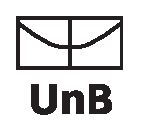
\includegraphics[width=1.5cm]{_extensions/nrennie/PrettyPDF/logo.eps}
          }%
     }%
}

%% Style the page number
\fancypagestyle{mystyle}{
  \fancyhf{}
  \renewcommand\headrulewidth{0pt}
  \fancyfoot[R]{\thepage}
  \fancyfootoffset{3.5cm}
}
\setlength{\footskip}{20pt}

%% style the chapter/section fonts
\chapterfont{\color{dark}\fontsize{20}{16.8}\selectfont}
\sectionfont{\color{dark}\fontsize{20}{16.8}\selectfont}
\subsectionfont{\color{dark}\fontsize{14}{16.8}\selectfont}
\titleformat{\subsection}
  {\sffamily\Large\bfseries}{\thesection}{1em}{}[{\titlerule[0.8pt]}]
  
% left align title
\makeatletter
\renewcommand{\maketitle}{\bgroup\setlength{\parindent}{0pt}
\begin{flushleft}
  {\sffamily\huge\textbf{\MakeUppercase{\@title}}} \vspace{1cm} \newline
  {\Large {\@subtitle}} \vspace{1cm} \newline
  \@author \newline
\end{flushleft}\egroup
}
\makeatother

%% Use some custom fonts
\setsansfont{Ubuntu}[
    Path=_extensions/nrennie/PrettyPDF/Ubuntu/,
    Scale=0.9,
    Extension = .ttf,
    UprightFont=*-Regular,
    BoldFont=*-Bold,
    ItalicFont=*-Italic,
    ]

\setmainfont{Ubuntu}[
    Path=_extensions/nrennie/PrettyPDF/Ubuntu/,
    Scale=0.9,
    Extension = .ttf,
    UprightFont=*-Regular,
    BoldFont=*-Bold,
    ItalicFont=*-Italic,
    ]
\KOMAoption{captions}{tableheading}
\makeatletter
\makeatother
\makeatletter
\@ifpackageloaded{bookmark}{}{\usepackage{bookmark}}
\makeatother
\makeatletter
\@ifpackageloaded{caption}{}{\usepackage{caption}}
\AtBeginDocument{%
\ifdefined\contentsname
  \renewcommand*\contentsname{Table of contents}
\else
  \newcommand\contentsname{Table of contents}
\fi
\ifdefined\listfigurename
  \renewcommand*\listfigurename{List of Figures}
\else
  \newcommand\listfigurename{List of Figures}
\fi
\ifdefined\listtablename
  \renewcommand*\listtablename{List of Tables}
\else
  \newcommand\listtablename{List of Tables}
\fi
\ifdefined\figurename
  \renewcommand*\figurename{Figure}
\else
  \newcommand\figurename{Figure}
\fi
\ifdefined\tablename
  \renewcommand*\tablename{Table}
\else
  \newcommand\tablename{Table}
\fi
}
\@ifpackageloaded{float}{}{\usepackage{float}}
\floatstyle{ruled}
\@ifundefined{c@chapter}{\newfloat{codelisting}{h}{lop}}{\newfloat{codelisting}{h}{lop}[chapter]}
\floatname{codelisting}{Listing}
\newcommand*\listoflistings{\listof{codelisting}{List of Listings}}
\makeatother
\makeatletter
\@ifpackageloaded{caption}{}{\usepackage{caption}}
\@ifpackageloaded{subcaption}{}{\usepackage{subcaption}}
\makeatother
\makeatletter
\@ifpackageloaded{tcolorbox}{}{\usepackage[skins,breakable]{tcolorbox}}
\makeatother
\makeatletter
\@ifundefined{shadecolor}{\definecolor{shadecolor}{rgb}{.97, .97, .97}}
\makeatother
\makeatletter
\@ifundefined{codebgcolor}{\definecolor{codebgcolor}{named}{light}}
\makeatother
\makeatletter
\makeatother
\ifLuaTeX
  \usepackage{selnolig}  % disable illegal ligatures
\fi
\IfFileExists{bookmark.sty}{\usepackage{bookmark}}{\usepackage{hyperref}}
\IfFileExists{xurl.sty}{\usepackage{xurl}}{} % add URL line breaks if available
\urlstyle{same} % disable monospaced font for URLs
\hypersetup{
  pdftitle={Prova 2 de Processo Estocásticos},
  pdfauthor={Professor Felipe Quintino},
  colorlinks=true,
  linkcolor={highlight},
  filecolor={Maroon},
  citecolor={Blue},
  urlcolor={highlight},
  pdfcreator={LaTeX via pandoc}}

\title{Prova 2 de Processo Estocásticos}
\usepackage{etoolbox}
\makeatletter
\providecommand{\subtitle}[1]{% add subtitle to \maketitle
  \apptocmd{\@title}{\par {\large #1 \par}}{}{}
}
\makeatother
\subtitle{Rafael de Acypreste (200060023) e Rafael Lira (190115858)}
\author{Professor Felipe Quintino}
\date{}

\begin{document}
\maketitle
\pagestyle{mystyle}

\ifdefined\Shaded\renewenvironment{Shaded}{\begin{tcolorbox}[sharp corners, breakable, borderline west={3pt}{0pt}{shadecolor}, frame hidden, colback={codebgcolor}, enhanced, boxrule=0pt]}{\end{tcolorbox}}\fi

\bookmarksetup{startatroot}

\hypertarget{prova-2-de-processo-estocuxe1sticos}{%
\chapter*{Prova 2 de Processo
Estocásticos}\label{prova-2-de-processo-estocuxe1sticos}}
\addcontentsline{toc}{chapter}{Prova 2 de Processo Estocásticos}

\markboth{Prova 2 de Processo Estocásticos}{Prova 2 de Processo
Estocásticos}

\hypertarget{aplicauxe7uxe3o-ao-modelo-empuxedrico}{%
\section*{Aplicação ao modelo
empírico}\label{aplicauxe7uxe3o-ao-modelo-empuxedrico}}
\addcontentsline{toc}{section}{Aplicação ao modelo empírico}

\markright{Aplicação ao modelo empírico}

Trata-se de um modelo para avaliar as probabilidades de transição entre
os estados de precipitação de chuvas.

\begin{Shaded}
\begin{Highlighting}[]
\CommentTok{\# Importing data}
\NormalTok{dados }\OtherTok{\textless{}{-}}
    \FunctionTok{read.delim}\NormalTok{(}\StringTok{"dados.txt"}\NormalTok{,}
        \AttributeTok{header =} \ConstantTok{TRUE}\NormalTok{,}
        \AttributeTok{sep    =} \StringTok{";"}
\NormalTok{    ) }\SpecialCharTok{|\textgreater{}}
    \FunctionTok{select}\NormalTok{(}\SpecialCharTok{{-}}\NormalTok{X) }\SpecialCharTok{|\textgreater{}}
    \FunctionTok{filter}\NormalTok{(}\SpecialCharTok{!}\FunctionTok{is.na}\NormalTok{(Precipitacao))}

\CommentTok{\# Summary statistics}
\NormalTok{dados}\SpecialCharTok{$}\NormalTok{Precipitacao }\SpecialCharTok{|\textgreater{}} \FunctionTok{summary}\NormalTok{()}
\end{Highlighting}
\end{Shaded}

\begin{verbatim}
   Min. 1st Qu.  Median    Mean 3rd Qu.    Max. 
  0.000   0.000   0.000   4.173   2.400 131.000 
\end{verbatim}

O primeiro passo é discretizar a variável de precipitação, que é feita
com a função \texttt{cut()} do pacote \texttt{base}. Para esse exemplo,
a variável será dividida em 3 categorias: sem chuva (precipitação até
\(0,1\)), chuva fraca (precipitação maior que \(0,1\) e menor que
\(10\)) e chuva forte.

\begin{Shaded}
\begin{Highlighting}[]
\CommentTok{\# Discretization of the variable}
\NormalTok{quantiles }\OtherTok{\textless{}{-}} \FunctionTok{quantile}\NormalTok{(dados}\SpecialCharTok{$}\NormalTok{Precipitacao,}
    \AttributeTok{probs =} \FunctionTok{seq}\NormalTok{(}\FloatTok{0.7}\NormalTok{, }\FloatTok{0.9}\NormalTok{, }\AttributeTok{length.out =} \DecValTok{3}\NormalTok{)}
\NormalTok{)}

\NormalTok{breaks }\OtherTok{\textless{}{-}} \FunctionTok{c}\NormalTok{(}\SpecialCharTok{{-}}\ConstantTok{Inf}\NormalTok{, }\FloatTok{0.001}\NormalTok{, quantiles, }\ConstantTok{Inf}\NormalTok{)}

\NormalTok{state\_labels }\OtherTok{\textless{}{-}} \FunctionTok{factor}\NormalTok{(}
    \FunctionTok{c}\NormalTok{(}
        \StringTok{"sem chuva"}\NormalTok{,}
        \StringTok{"garoa"}\NormalTok{,}
        \StringTok{"chuva fraca"}\NormalTok{,}
        \StringTok{"chuva moderada"}\NormalTok{,}
        \StringTok{"chuva forte"}
\NormalTok{    ),}
    \AttributeTok{levels =} \FunctionTok{c}\NormalTok{(}
        \StringTok{"sem chuva"}\NormalTok{,}
        \StringTok{"garoa"}\NormalTok{,}
        \StringTok{"chuva fraca"}\NormalTok{,}
        \StringTok{"chuva moderada"}\NormalTok{,}
        \StringTok{"chuva forte"}
\NormalTok{    )}
\NormalTok{)}

\CommentTok{\# Discretization}
\NormalTok{dados }\OtherTok{\textless{}{-}}
\NormalTok{    dados }\SpecialCharTok{|\textgreater{}}
    \CommentTok{\# Discretization}
    \FunctionTok{mutate}\NormalTok{(}\AttributeTok{rain\_status =} \FunctionTok{cut}\NormalTok{(Precipitacao,}
        \AttributeTok{breaks =}\NormalTok{ breaks,}
        \AttributeTok{labels =}\NormalTok{ state\_labels}
\NormalTok{    ))}
\end{Highlighting}
\end{Shaded}

Para esse exemplo, serão separadas as 10 últimas observações para
avaliar as estimações.

\begin{Shaded}
\begin{Highlighting}[]
\NormalTok{dados\_teste }\OtherTok{\textless{}{-}} \FunctionTok{tail}\NormalTok{(dados, }\DecValTok{10}\NormalTok{)}
\NormalTok{dados\_treinamento }\OtherTok{\textless{}{-}}\NormalTok{ dados[}\DecValTok{1}\SpecialCharTok{:}\NormalTok{(}\FunctionTok{nrow}\NormalTok{(dados) }\SpecialCharTok{{-}} \DecValTok{10}\NormalTok{), ]}
\end{Highlighting}
\end{Shaded}

Para estimar as transições de estado, é necessário criar uma variável
que identifique o estado atual e o estado seguinte. Para isso, é
necessário criar uma variável defasada, que pode ser feita com a função
\texttt{lag()} do pacote \texttt{dplyr}. Depois disso, basta avaliar as
proporções das transições de estado.

\begin{Shaded}
\begin{Highlighting}[]
\CommentTok{\# Creating the lagged variable}
\NormalTok{transicoes\_chuva }\OtherTok{\textless{}{-}}
\NormalTok{    dados\_treinamento }\SpecialCharTok{|\textgreater{}}
    \CommentTok{\# Lag variable}
    \FunctionTok{mutate}\NormalTok{(}\AttributeTok{rain\_status\_lag =} \FunctionTok{lag}\NormalTok{(rain\_status)) }\SpecialCharTok{|\textgreater{}}
    \CommentTok{\# Exclude the last state}
    \FunctionTok{filter}\NormalTok{(}\SpecialCharTok{!}\FunctionTok{is.na}\NormalTok{(rain\_status\_lag)) }\SpecialCharTok{|\textgreater{}}
    \CommentTok{\# Count the transitions}
    \FunctionTok{count}\NormalTok{(rain\_status, rain\_status\_lag) }\SpecialCharTok{|\textgreater{}}
    \CommentTok{\# Calculates the estimator}
    \FunctionTok{mutate}\NormalTok{(}
        \AttributeTok{Prop =} \FunctionTok{round}\NormalTok{(n }\SpecialCharTok{/} \FunctionTok{sum}\NormalTok{(n), }\AttributeTok{digits =} \DecValTok{3}\NormalTok{),}
        \AttributeTok{.by =}\NormalTok{ rain\_status}
\NormalTok{    )}
\end{Highlighting}
\end{Shaded}

A matriz de transição estimada entre os estados sem chuva, garoa, chuva
fraca, chuva moderada, chuva forte, nesta ordem, é dada por:

\begin{equation}
P =
\begin{pmatrix}
0.822 & 0.041 &  0.051 & 0.045 &  0.04 \\
0.334 & 0.12 &  0.186 & 0.177 &  0.183 \\
0.306 & 0.133 &  0.187 & 0.184 &  0.19 \\
0.306 & 0.121 &  0.171 & 0.193 &  0.21 \\
0.282 & 0.118 &  0.174 & 0.204 &  0.223 
\end{pmatrix}
\end{equation}

Agora, pode-se recuperar a matriz de transição para fazer as estimativas
de transição de estado.

\begin{Shaded}
\begin{Highlighting}[]
\CommentTok{\# Transition matrix}
\NormalTok{matriz\_transicao }\OtherTok{\textless{}{-}}
\NormalTok{    transicoes\_chuva }\SpecialCharTok{|\textgreater{}}
    \FunctionTok{select}\NormalTok{(}\SpecialCharTok{{-}}\NormalTok{n) }\SpecialCharTok{|\textgreater{}}
    \FunctionTok{pivot\_wider}\NormalTok{(}
        \AttributeTok{names\_from =}\NormalTok{ rain\_status\_lag,}
        \AttributeTok{values\_from =}\NormalTok{ Prop}
\NormalTok{    ) }\SpecialCharTok{|\textgreater{}}
    \FunctionTok{column\_to\_rownames}\NormalTok{(}\StringTok{"rain\_status"}\NormalTok{) }\SpecialCharTok{|\textgreater{}}
    \FunctionTok{as.matrix}\NormalTok{()}

\NormalTok{ultimo\_estado }\OtherTok{\textless{}{-}}\NormalTok{ dados\_treinamento }\SpecialCharTok{|\textgreater{}}
    \FunctionTok{tail}\NormalTok{(}\DecValTok{1}\NormalTok{) }\SpecialCharTok{|\textgreater{}}
    \FunctionTok{pull}\NormalTok{(rain\_status)}
\end{Highlighting}
\end{Shaded}

Com a matriz de transição, basta considerar o último estado dos dados
(garoa) ---- consequência da propriedade de Markov ---- de treinamento
para fazer as estimativas de transição de estado.

\begin{Shaded}
\begin{Highlighting}[]
\NormalTok{simula\_cadeia\_markov }\OtherTok{\textless{}{-}} \ControlFlowTok{function}\NormalTok{(}\AttributeTok{n =} \DecValTok{10}\NormalTok{,}
\NormalTok{                                 valor\_inicial,}
\NormalTok{                                 matriz\_transicao,}
\NormalTok{                                 estados) \{}
\NormalTok{    P }\OtherTok{\textless{}{-}}\NormalTok{ matriz\_transicao}
\NormalTok{    y }\OtherTok{\textless{}{-}}\NormalTok{ valor\_inicial}

    \CommentTok{\# Simulation of the stochastic process}
    \ControlFlowTok{for}\NormalTok{ (i }\ControlFlowTok{in} \DecValTok{1}\SpecialCharTok{:}\NormalTok{n) \{}
        \CommentTok{\# Sample of the next state}
\NormalTok{        y[i }\SpecialCharTok{+} \DecValTok{1}\NormalTok{] }\OtherTok{\textless{}{-}} \FunctionTok{sample}\NormalTok{(estados, }\AttributeTok{size =} \DecValTok{1}\NormalTok{, }\AttributeTok{prob =}\NormalTok{ P[y[i], ])}
\NormalTok{    \}}

    \FunctionTok{return}\NormalTok{(y[}\SpecialCharTok{{-}}\DecValTok{1}\NormalTok{])}
\NormalTok{\}}
\CommentTok{\# Excecution of the function}
\NormalTok{previsoes }\OtherTok{\textless{}{-}} \FunctionTok{simula\_cadeia\_markov}\NormalTok{(}
    \AttributeTok{valor\_inicial =}\NormalTok{ ultimo\_estado,}
    \AttributeTok{matriz\_transicao =}\NormalTok{ matriz\_transicao,}
    \AttributeTok{estados =}\NormalTok{ state\_labels,}
    \AttributeTok{n =} \DecValTok{10}
\NormalTok{)}
\end{Highlighting}
\end{Shaded}

E, então, pode-se comparar as previsões com os dados de teste. Para o
gráfico, os acertos são indicados pela linha tracejada vermelha.

\begin{Shaded}
\begin{Highlighting}[]
\NormalTok{comparacao }\OtherTok{\textless{}{-}}
    \FunctionTok{data.frame}\NormalTok{(}
        \AttributeTok{observado =}\NormalTok{ dados\_teste}\SpecialCharTok{$}\NormalTok{rain\_status,}
        \AttributeTok{previsao =}\NormalTok{ previsoes}
\NormalTok{    )}

\CommentTok{\# Imprime a tabela}
\NormalTok{comparacao}
\end{Highlighting}
\end{Shaded}

\begin{verbatim}
        observado       previsao
1  chuva moderada chuva moderada
2  chuva moderada    chuva fraca
3     chuva forte chuva moderada
4       sem chuva          garoa
5       sem chuva    chuva fraca
6       sem chuva      sem chuva
7       sem chuva      sem chuva
8       sem chuva      sem chuva
9     chuva fraca      sem chuva
10          garoa    chuva forte
\end{verbatim}

\begin{Shaded}
\begin{Highlighting}[]
\CommentTok{\# Constroi o gráfico}
\NormalTok{comparacao }\SpecialCharTok{|\textgreater{}}
    \FunctionTok{ggplot}\NormalTok{(}\FunctionTok{aes}\NormalTok{(}\AttributeTok{x =}\NormalTok{ observado, }\AttributeTok{y =}\NormalTok{ previsao)) }\SpecialCharTok{+}
    \FunctionTok{geom\_jitter}\NormalTok{(}
        \AttributeTok{size =} \DecValTok{3}\NormalTok{, }\AttributeTok{shape =} \DecValTok{2}\NormalTok{,}
        \AttributeTok{width =} \FloatTok{0.15}\NormalTok{, }\AttributeTok{height =} \FloatTok{0.15}
\NormalTok{    ) }\SpecialCharTok{+}
    \FunctionTok{geom\_abline}\NormalTok{(}
        \AttributeTok{intercept =} \DecValTok{0}\NormalTok{,}
        \AttributeTok{slope =} \DecValTok{1}\NormalTok{,}
        \AttributeTok{color =} \StringTok{"red"}\NormalTok{,}
        \AttributeTok{linetype =} \StringTok{"dashed"}
\NormalTok{    ) }\SpecialCharTok{+}
    \FunctionTok{theme\_bw}\NormalTok{() }\SpecialCharTok{+}
    \FunctionTok{labs}\NormalTok{(}
        \AttributeTok{x =} \StringTok{"Observado"}\NormalTok{,}
        \AttributeTok{y =} \StringTok{"Previsão"}\NormalTok{,}
        \AttributeTok{title =} \StringTok{"Previsões vs. Observações"}
\NormalTok{    )}
\end{Highlighting}
\end{Shaded}

\begin{figure}[H]

{\centering 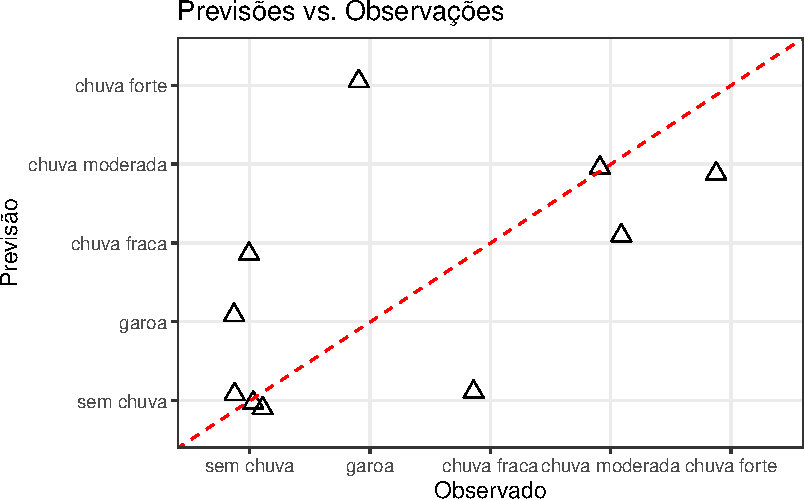
\includegraphics{index_files/figure-pdf/unnamed-chunk-8-1.pdf}

}

\end{figure}

\bookmarksetup{startatroot}

\hypertarget{questuxe3o-2}{%
\chapter*{Questão 2}\label{questuxe3o-2}}
\addcontentsline{toc}{chapter}{Questão 2}

\markboth{Questão 2}{Questão 2}

Espaço para a resposta da questão 2



\printindex

\end{document}
